\documentclass[10pt,a4paper]{article}
\usepackage[margin=2.2cm]{geometry}
\usepackage[T1]{fontenc}
\usepackage{lmodern}
\usepackage{parskip}
\usepackage{booktabs}
\usepackage{tabularx}
\usepackage{array}
\usepackage{float}
\usepackage{graphicx}
\usepackage{enumitem}
\usepackage{xcolor}
\usepackage{xurl}
\usepackage[colorlinks=true,urlcolor=blue!60!black,linkcolor=black]{hyperref}

\graphicspath{{../telemetry_bench_20261124_223344/figures/}}
\newcolumntype{R}{>{\raggedleft\arraybackslash}X}

\title{Drone Authentication Study --- Step 5 Progress Report\\[3pt]
\large Signed sensor telemetry (MPU6050) on the ESP32}
\author{}
\date{24 November 2026}

\begin{document}
\maketitle

\section*{Summary}

A drone sends its sensor readings (accelerometer and gyroscope) to the ground station many times
per second. In Step 5 we measured what it costs the ESP32 to sign these readings, with every
algorithm, at 10, 50 and 100 readings per second. The results:

\begin{enumerate}[nosep]
  \item \textbf{Only Ed25519 can sign every reading in real time.} One signature takes 9.6\,ms, so it
        keeps up even at 100 readings per second. One by one, ML-DSA-44 manages about 13 per second,
        ECDSA 6, ML-DSA-87 5 and RSA-3072 about 3. ML-DSA-44 is faster than ECDSA and RSA here.
  \item \textbf{Signing 10 readings together fixes the speed problem for ML-DSA-44}: at 100 readings
        per second it signed 99\% of them. The price is older data (0.18\,s typical).
  \item \textbf{ML-DSA sometimes takes much longer} (up to 0.25--0.86\,s for one signature instead
        of about 0.05--0.14\,s), so some readings are up to about 1\,s old when they are signed.
  \item \textbf{Signing does not disturb the sensor, if the firmware is built correctly.} With the
        sensor in its own high-priority task, every reading was taken at most 47\,\textmu s late,
        with every algorithm. If reading and signing are done in one simple loop, the drone
        \textbf{misses 76--95\%} of its readings with the slow algorithms.
  \item \textbf{The radio is the real limit.} On a typical 57,600-baud drone radio, readings signed one
        by one with ML-DSA-44 fit only about 2 times per second (21 with 10 readings per signature),
        against 54 for Ed25519.
  \item \textbf{MAVLink 2's own signing}, which drones use today, takes only 0.05\,ms and 13 bytes, but
        it needs a key shared in advance. Best design: \textbf{ML-DSA-44 to authenticate the drone once,
        then MAVLink 2 signing for the telemetry.}
\end{enumerate}

% ---------------------------------------------------------------------------
\section{What we did}

\begin{itemize}[nosep]
  \item \textbf{Board:} the same ESP32 (240\,MHz) and the same six algorithms as in Steps 1--3. No
        Wi-Fi: the network was measured in Step 3.
  \item \textbf{Sensor data:} our MPU6050 did not answer on the I2C bus, so the firmware used
        \textbf{simulated readings}: the same 14 bytes, in the same order, as a real MPU6050 reading
        (accelerometer, temperature, gyroscope), with realistic values. A signature only depends on how
        many bytes are signed, not on what they say, so the timings are the same as with a real sensor.
        The firmware uses a real MPU6050 automatically when one is connected.
  \item \textbf{One reading} = 22 bytes: reading number (4), drone clock (4), sensor bytes (14). A
        message has an 8-byte header, the readings, then the signature.
  \item \textbf{Three ways to protect the readings:}
        \begin{itemize}[nosep]
          \item \emph{every reading signed} on its own (1 reading per message);
          \item \emph{10 readings per signature} (the drone collects 10, then signs them together);
          \item \emph{MAVLink 2 signing}: the 13-byte signature that the MAVLink drone protocol adds to
                every packet, made with a key shared by the drone and the ground station
                (\url{https://mavlink.io/en/guide/message_signing.html}).
        \end{itemize}
  \item \textbf{How the firmware is built:} a high-priority \emph{sensor task} takes a reading at
        exact times (a hardware timer) and puts it in a buffer; a lower-priority \emph{signing task}
        signs what is in the buffer. The buffer keeps at most 0.5\,s of unsigned readings: when the
        signing task cannot keep up, the oldest readings are thrown away, so the drone always signs
        fresh data. For comparison we also ran a \emph{simple loop} (read, then sign, then read again),
        the way a beginner's Arduino sketch would do it.
  \item \textbf{Each run} lasted 10 seconds; 49 runs in total. Every algorithm first passed its
        known-answer test, and the last signed message of every run was checked.
\end{itemize}

\textbf{What we measured} in every run:
\begin{description}[nosep,leftmargin=1.2em,font=\normalfont\bfseries]
  \item[Signed readings] how many readings per second got a signature.
  \item[Age] how old the oldest reading in a message is when its signature is ready (how fresh the
        data is when it can be sent).
  \item[Late] how late each reading was taken compared with its exact time (does signing disturb the
        sensor?).
  \item[Missed] readings that were not taken at all because the simple loop was busy signing.
\end{description}

% ---------------------------------------------------------------------------
\section{How many readings per second can be signed}

\begin{figure}[H]
  \centering
  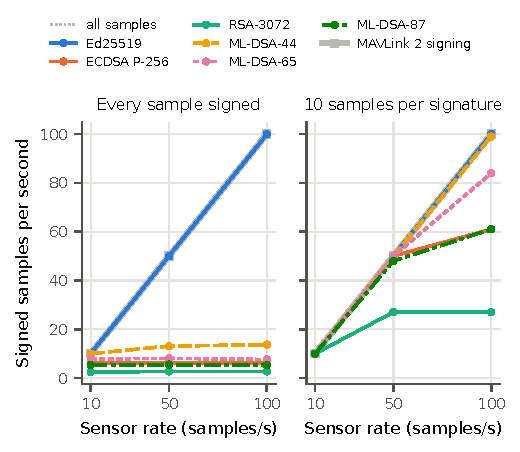
\includegraphics[width=0.56\linewidth]{fig11_signed_rate.pdf}
  \caption{Signed readings per second at each sensor rate. The dotted line means ``all readings
  signed''. Left: every reading signed on its own. Right: 10 readings per signature.}
\end{figure}

\begin{table}[H]
\centering\small
\begin{tabularx}{0.95\textwidth}{@{}l RR RR@{}}
\toprule
 & \multicolumn{2}{c}{\textbf{Time for one signature}} & \multicolumn{2}{c}{\textbf{Signed per second at 100/s}} \\
\cmidrule(lr){2-3}\cmidrule(l){4-5}
Algorithm & Typical & Slow (p99) & Every reading & 10 per signature \\
\midrule
Ed25519          & 9.6\,ms   & 9.6\,ms   & \textbf{100} (all) & \textbf{100} (all) \\
ECDSA P-256      & 162\,ms   & 164\,ms   & 6.2  & 61 \\
RSA-3072         & 374\,ms   & 378\,ms   & 2.7  & 27 \\
ML-DSA-44        & 52\,ms    & 376\,ms   & 13.7 & \textbf{99} \\
ML-DSA-65        & 104\,ms   & 661\,ms   & 7.6  & 84 \\
ML-DSA-87        & 141\,ms   & 744\,ms   & 5.3  & 61 \\
MAVLink 2 signing & 0.05\,ms & 0.05\,ms  & \textbf{100} (all) & --- \\
\bottomrule
\end{tabularx}
\caption{Signing speed in Step 5. ``Slow (p99)'': 1 signature in 100 takes this long or longer.
The signing times match Step 1 (Ed25519 9.4\,ms, ML-DSA-44 55\,ms there). RSA-3072: one
signature, in the 10-per-second run, took 967\,ms.}
\end{table}

\textbf{What it means:}
\begin{itemize}[nosep]
  \item To sign every reading at $N$ readings per second, one signature must take less than $1/N$
        seconds: 100\,ms at 10/s, 20\,ms at 50/s, 10\,ms at 100/s. Only Ed25519 (9.6\,ms) and MAVLink
        signing meet this at every rate.
  \item ML-DSA-44 signs about twice as many readings as ECDSA and five times as many as RSA, but it is
        still far from 50 or 100 per second.
  \item Signing 10 readings together costs almost the same time as signing one, so it gives about ten
        times more signed readings. With it, ML-DSA-44 handles 100 readings per second.
\end{itemize}

% ---------------------------------------------------------------------------
\section{How fresh is the signed data?}

\begin{figure}[H]
  \centering
  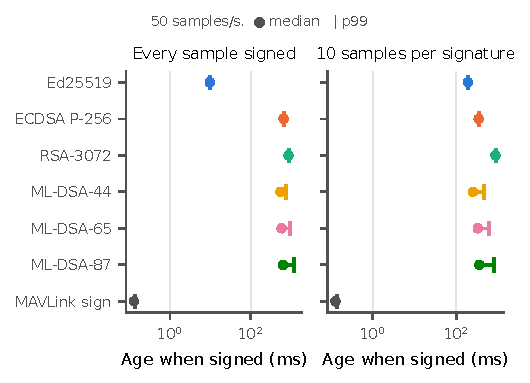
\includegraphics[width=0.56\linewidth]{fig12_age.pdf}
  \caption{Age of the data when its signature is ready, at 50 readings per second (log scale). Dot:
  typical (median); bar: slow case (p99).}
\end{figure}

\begin{table}[H]
\centering\small
\begin{tabularx}{\textwidth}{@{}l RRR RRR@{}}
\toprule
 & \multicolumn{3}{c}{\textbf{Every reading signed}} & \multicolumn{3}{c}{\textbf{10 readings per signature}} \\
\cmidrule(lr){2-4}\cmidrule(l){5-7}
Algorithm & Signed & Age typical & Age slow & Signed & Age typical & Age slow \\
\midrule
Ed25519           & 100\%  & 10\,ms  & 10\,ms    & 100\% & 190\,ms & 190\,ms \\
ECDSA P-256       & 12\%   & 652\,ms & 662\,ms   & 100\% & 342\,ms & 343\,ms \\
RSA-3072          & 5\%    & 864\,ms & 875\,ms   & 54\%  & 863\,ms & 874\,ms \\
ML-DSA-44         & 26\%   & 546\,ms & 766\,ms   & 100\% & 250\,ms & 462\,ms \\
ML-DSA-65         & 16\%   & 584\,ms & 918\,ms   & 100\% & 327\,ms & 614\,ms \\
ML-DSA-87         & 11\%   & 631\,ms & 1,193\,ms & 96\%  & 356\,ms & 789\,ms \\
MAVLink 2 signing & 100\%  & 0.13\,ms & 0.14\,ms & ---   & ---     & ---     \\
\bottomrule
\end{tabularx}
\caption{At 50 readings per second. ``Slow'' = p99. ML-DSA-87 with 10 per signature: no reading was
thrown away; the last 4\% were still waiting when the 10-second run ended.}
\end{table}

\textbf{What it means:}
\begin{itemize}[nosep]
  \item When an algorithm cannot keep up, the buffer stays full and the signed data is about 0.5\,s old
        (the buffer length) plus the signing time. That is why the slow algorithms show 0.5--0.9\,s.
  \item With 10 readings per signature, the first reading of a message has to wait for the other 9:
        180\,ms at 50 readings per second, before signing even starts.
  \item ML-DSA's slow cases come from how ML-DSA works: it tries a signature, checks it, and starts again
        if the check fails, a random number of times. Most signatures need few tries, a few need many.
\end{itemize}

% ---------------------------------------------------------------------------
\section{Does signing disturb the sensor?}

\begin{figure}[H]
  \centering
  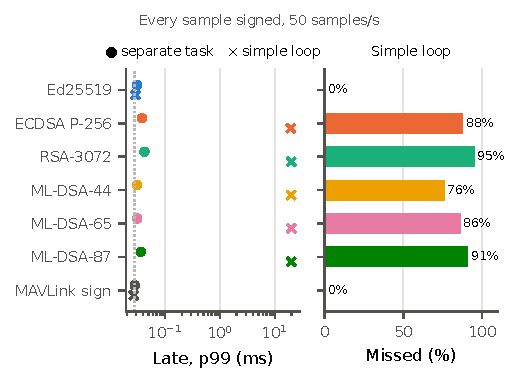
\includegraphics[width=0.56\linewidth]{fig13_sampling.pdf}
  \caption{Every reading signed, 50 readings per second. Left: how late the readings were taken (slow
  case, p99, log scale), with a separate sensor task (dots) and in a simple loop (crosses); the dotted
  line is the sensor alone, without any signing. Right: readings missed by the simple loop.}
\end{figure}

\begin{table}[H]
\centering\small
\begin{tabularx}{0.85\textwidth}{@{}l RRR@{}}
\toprule
 & \textbf{Separate sensor task} & \multicolumn{2}{c}{\textbf{Simple loop}} \\
\cmidrule(lr){2-2}\cmidrule(l){3-4}
Algorithm & Latest reading & Readings missed & Latest reading \\
\midrule
No signing (sensor alone) & 41\,\textmu s & --- & --- \\
Ed25519           & 34\,\textmu s & 0\%    & 29\,\textmu s \\
ECDSA P-256       & 40\,\textmu s & 87.8\% & 19.4\,ms \\
RSA-3072          & 47\,\textmu s & 95.0\% & 19.8\,ms \\
ML-DSA-44         & 41\,\textmu s & 76.0\% & 19.9\,ms \\
ML-DSA-65         & 31\,\textmu s & 86.2\% & 19.8\,ms \\
ML-DSA-87         & 36\,\textmu s & 91.0\% & 19.8\,ms \\
MAVLink 2 signing & 28\,\textmu s & 0\%    & 27\,\textmu s \\
\bottomrule
\end{tabularx}
\caption{Separate sensor task: the latest reading over all runs and rates of that algorithm. Simple
loop: 50 readings per second, every reading signed.}
\end{table}

\textbf{What it means:}
\begin{itemize}[nosep]
  \item With a separate high-priority sensor task, signing does not disturb the sensor at all: readings
        are at most 47\,\textmu s late with every algorithm, almost the same as without signing
        (28--41\,\textmu s). The processor simply pauses the signing whenever a reading is due.
  \item In a simple loop, the sensor has to wait until the signature is finished. Every algorithm that
        takes longer than one reading period (20\,ms at 50 per second) loses most readings: 76\% with
        ML-DSA-44, up to 95\% with RSA.
  \item So the firmware design matters as much as the algorithm: \textbf{signing must run in its own
        lower-priority task.}
\end{itemize}

% ---------------------------------------------------------------------------
\section{Can the radio carry it?}

\begin{figure}[H]
  \centering
  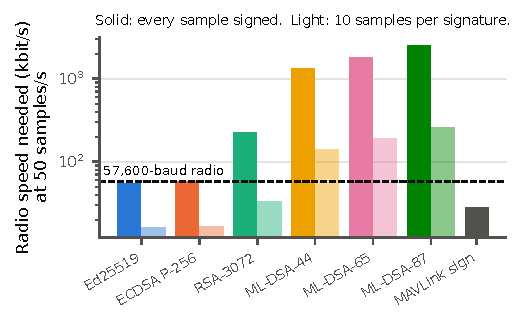
\includegraphics[width=0.56\linewidth]{fig14_radio.pdf}
  \caption{Radio speed needed to send 50 signed readings per second in MAVLink 2 packets (log scale),
  compared with a 57,600-baud drone telemetry radio. Calculated from the measured message sizes.}
\end{figure}

\begin{table}[H]
\centering\small
\begin{tabularx}{0.9\textwidth}{@{}l RR RR@{}}
\toprule
 & \multicolumn{2}{c}{\textbf{Every reading signed}} & \multicolumn{2}{c}{\textbf{10 readings per signature}} \\
\cmidrule(lr){2-3}\cmidrule(l){4-5}
Algorithm & Bytes per reading & Max readings/s & Bytes per reading & Max readings/s \\
\midrule
Ed25519           & 106   & 54   & 32  & 182 \\
ECDSA P-256       & 113   & 51   & 32  & 179 \\
RSA-3072          & 438   & 13   & 65  & 89 \\
ML-DSA-44         & 2,570 & 2.2  & 278 & 21 \\
ML-DSA-65         & 3,507 & 1.6  & 370 & 16 \\
ML-DSA-87         & 4,885 & 1.2  & 510 & 11 \\
MAVLink 2 signing & 55    & 105  & --- & --- \\
\bottomrule
\end{tabularx}
\caption{Bytes on the radio per reading (message + signature + 12 bytes of MAVLink 2 header and
checksum per packet) and the most readings per second a 57,600-baud radio can carry (5,760 bytes
per second: 10 bits per byte on a serial line). Calculated, not measured on a real radio.}
\end{table}

\textbf{What it means:} even where the ESP32 is fast enough, an ML-DSA signature on every reading
does not fit on a drone radio: one ML-DSA-44 signature is 2,420 bytes, 110 times the reading it protects.
With 10 readings per signature, ML-DSA-44 fits about 21 readings per second, which is enough for slow
telemetry (position, battery) but not for fast attitude data.

% ---------------------------------------------------------------------------
\section{What we learn from Step 5}

\begin{enumerate}[nosep]
  \item \textbf{Post-quantum signatures cannot protect every telemetry message} on an ESP32 drone with a
        normal radio: ML-DSA is too slow to sign every reading and far too big to send with every
        reading.
  \item \textbf{ML-DSA-44 is the best post-quantum choice}: it signs faster than ML-DSA-65/87, and even
        faster than ECDSA and RSA, but its occasional slow signatures must be planned for.
  \item \textbf{The practical design is hybrid:} the drone proves who it is \emph{once} with an ML-DSA-44
        signature (Steps 3 and 4: about 91\,ms on Wi-Fi), and the readings are then protected with
        MAVLink 2 signing using a shared key (0.05\,ms and 13 bytes per packet). MAVLink itself says
        this key must be set up over a secure link; to keep it safe against quantum computers too, it
        should be agreed with a post-quantum key exchange such as ML-KEM, which our PQC VPN already uses.
  \item \textbf{Signing must run in its own lower-priority task}, or the drone loses most of its sensor
        readings.
\end{enumerate}

\textbf{Limits.} Simulated sensor data (the MPU6050 did not answer; timings do not depend on the data
values); one board; 10 seconds per run; radio figures are calculated, not measured on a real radio.

\textbf{Files.} {\small\ttfamily firmware/sig\_bench\_unified/e5\_telemetry.ino} (send T);\\
log {\small\ttfamily results/e5/raw/telemetry\_bench\_20261124\_223344.log};\\
tables and figures {\small\ttfamily results/e5/telemetry\_bench\_20261124\_223344/}; analysis
{\small\ttfamily tools/analyze\_telemetry.py}.

\end{document}
